 %\newpage
%\pagestyle{empty}

\chapter{INTRODUÇÃO}{}

 \section{Introdução}

A bananicultura é uma das atividades agrícolas de maior importância econômica e social no Brasil. O país ocupa a quinta posição entre os maiores produtores mundiais de banana. No mercado interno, a fruta se destaca como a segunda mais relevante, após a laranja, em área colhida (460 mil hectares em 2023), quantidade produzida (6,8 milhões de toneladas) e valor de produção (13,8 bilhões de reais) \cite{KULEF2024}. Além disso, é uma das frutas mais consumidas no país, com um consumo aparente de aproximadamente 25 kg por habitante ao ano \cite{KULEF2024}.

A banana é cultivada em todo o território nacional, com destaque para as regiões Nordeste e Sudeste, que juntas representam cerca de 70\% da área cultivada e da produção, e aproximadamente 65\% do valor da produção nacional \cite{KULEF2024}. No Nordeste, destacam-se os estados da Bahia  especialmente os municípios de Bom Jesus da Lapa, no Oeste Baiano, e o Sul do estado  e Pernambuco, com a Zona da Mata e a microrregião de Petrolina.

O município de Bom Jesus da Lapa tem ganhado destaque como um dos principais polos produtores de banana do país. Em 2023, foi o maior produtor nacional, com uma área implantada de 12.715,7 hectares e produtividade média de 22,7 toneladas por hectare. Neste mesmo ano, o município foi responsável por cerca de 20\% da produção baiana. O cultivo é realizado com elevado nível tecnológico no perímetro irrigado Formoso, onde, segundo a Codevasf (2024), a banana ocupou 88\% da área cultivada e respondeu por 91\% do valor da produção agrícola no perímetro.

Além do perímetro irrigado Formoso, outros perímetros públicos de irrigação no Médio São Francisco, na Bahia, também apresentam expressiva produção de banana: Barreiras Norte (83\%), Ceraíma (51\%), Estreito (65\%), Mirorós (91\%), Nupeba (82\%), Piloto Formoso (98\%), Riacho Grande (77\%) e São Desidério Barreiras Sul (10\%) \cite{Codevasf2024}.

Apesar da relevância da atividade, a bananicultura brasileira enfrenta diversos desafios, especialmente no controle de doenças. As principais variedades cultivadas no país, como a banana prata e maçã, são suscetíveis a diversas doenças foliares, como a sigatoka amarela, sigatoka negra, mancha foliar de Cordana e a Pestalotiopsis palmarum \cite{KULEF2024}, todas causadas por fungos que afetam as folhas, comprometendo a fotossíntese e reduzindo a produtividade. Outra doença de grande impacto é o Mal do Panamá, também de origem fúngica, que atinge o sistema vascular da planta, provocando murcha e morte dos pés de bananeira \cite{CORDEIRO2017}.

O monitoramento eficiente das plantações é essencial para conter a disseminação dessas doenças e permitir ações de controle rápidas e eficazes. No entanto, os métodos tradicionais de identificação, que dependem da atuação de especialistas ou de análises laboratoriais, são geralmente demorados e onerosos, o que dificulta sua aplicação em regiões rurais mais afastadas. Nesse cenário, o uso de tecnologias baseadas em Inteligência Computacional (IC), como a visão computacional e o Aprendizado Profundo (AP), tem se mostrado uma alternativa promissora \cite{ZHANG2022, REZENDE2019}.

Diversos estudos têm sido conduzidos com o objetivo de prever incidentes e minimizar perdas na agricultura por meio de técnicas de IC, especialmente utilizando aprendizado profundo e visão computacional para reconhecimento de padrões em imagens de doenças em plantas \cite{GANDHI2018, LIU2017, MOHANTY2016}. Dentre as várias arquiteturas de redes neurais utilizadas, as redes neurais convolucionais (Convolutional Neural Networks — CNNs) destacam-se pelo seu desempenho superior em tarefas de reconhecimento de objetos visuais \cite{OLIVEIRA2018, PENHA2018, TODA2019}, resultado que tem sido impulsionado pelos avanços no processamento computacional, especialmente com o uso de GPUs (Graphics Processing Units).

Pesquisas recentes também têm explorado o desenvolvimento de dispositivos automáticos que aplicam técnicas de processamento de imagens para apoiar a tomada de decisão na identificação de doenças que afetam o cultivo da banana \cite{IBARRA2023}. Nesse contexto, destacam-se os algoritmos de Aprendizado Profundo e visão computacional, capazes de reconhecer padrões em grandes bases de dados de imagens \cite{REZENDE2019}.

AJUSTAR CONFORME O QUE FOI REALIZADO NO TRABALHO E AS ANALISES FEITA SDO S RESULTADOS E METODOLOGIA IMPLEMENTADA

\textbf{\textit{Neste trabalho, propõe-se o desenvolvimento de uma rede neural convolucional para a classificação de doenças foliares em plantas de banana. O modelo será treinado a partir da base de dados \textit{BananaLSD}, disponibilizada por \cite{ARMAN2023}, contendo imagens de folhas afetadas por sigatoka, mancha foliar de Cordana, Pestalotiopsis e folhas sadias. Serão criadas dez bases de dados distintas, variando em número de classes e resoluções de imagens. A avaliação do desempenho do modelo será feita por meio de métricas consolidadas como acurácia na etapa de teste, F1-score e área sob a curva (AUC). Para complementar, será aplicado um teste estatístico não paramétrico com base na acurácia, a fim de verificar a significância dos resultados obtidos.}}




%\thispagestyle{empty}
%\pagestyle{fancy}
\section{Objetivos}


Desenvolver um sistema de classificação de doenças em plantações de bananeiras utilizando redes neurais convolucionais, por meio da análise de imagens foliares.


\subsection{Objetivos Específicos}
    \begin{itemize}
      \item Realizar o preparo e o pré-processamento das imagens da base de dados utilizada;
      \item Implementar uma rede neural convolucional para classificação de doenças foliares em bananeiras;
      \item Realizar a identificação das principais doenças da cultura da banana presentes nas imagens;
      \item Avaliar o desempenho do modelo por meio de métricas como acurácia e taxa de erro.
    \end{itemize}

\section{Metodologia da Pesquisa}

A metodologia de implementação desta proposta resulta no entendimento acerca da problemática, assim pretende-se dividir em três etapas distintas: 


% \begin{figure}[!h]
% 	\centering
% 	\caption{Etapas para o desenvolvimento da metodologia científica}
% 	%\vskip 5mm
% 	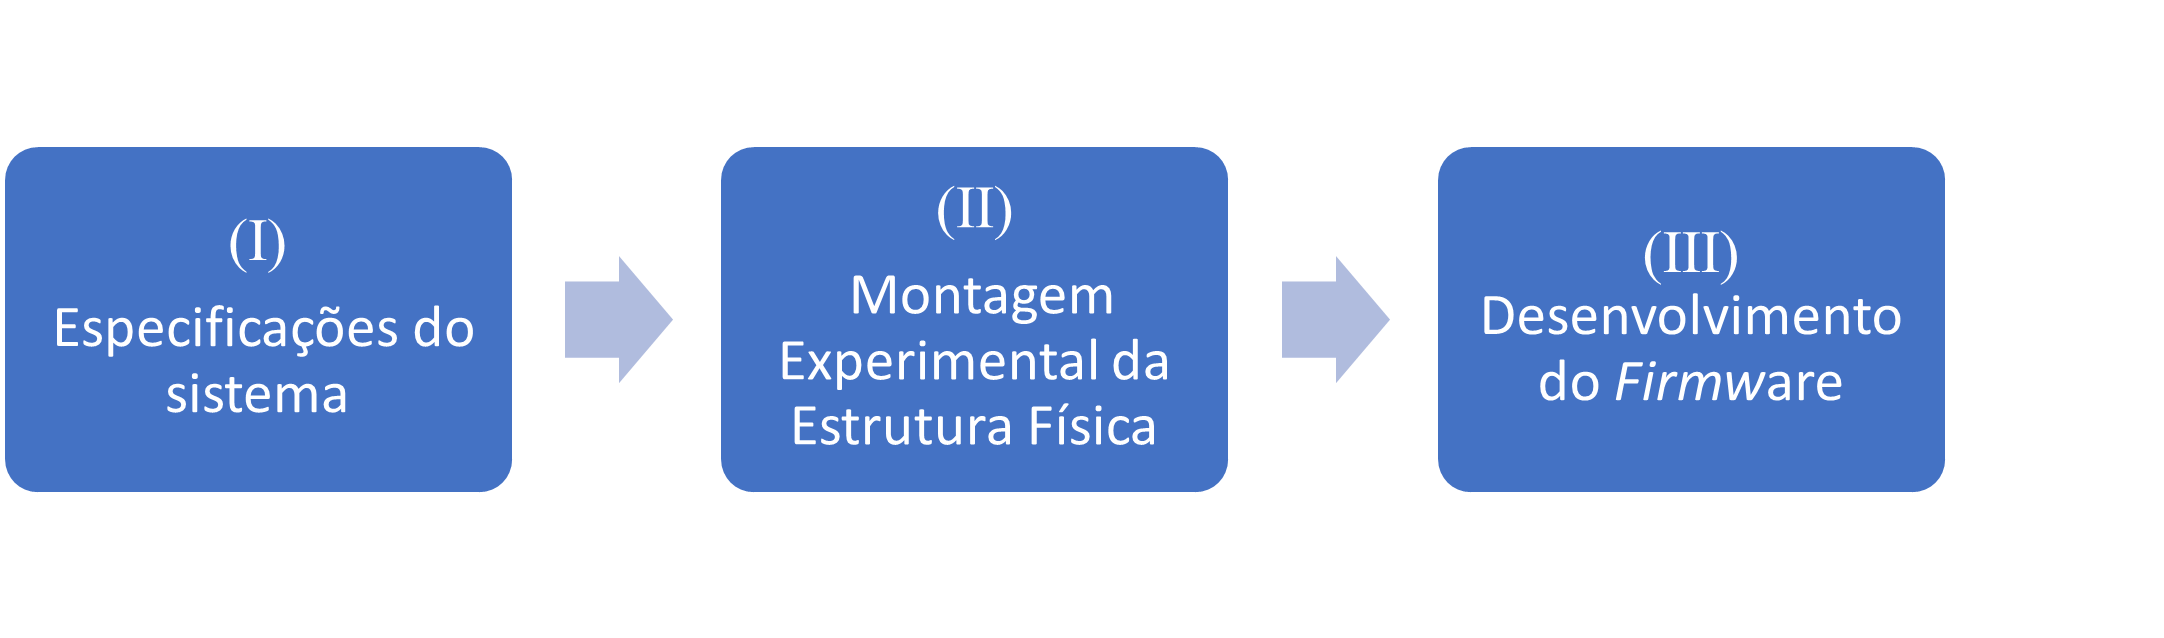
\includegraphics[width=16cm]{figuras/Metodologia.png}\\
% 	\autoria{Autoria Própria (2022)}
% 	\label{fig:Metodologia}
% \end{figure}

A metodologia adotada para o desenvolvimento do \textit{Sistema de Classificação de Doenças em Plantações de Bananeiras Utilizando Redes Neurais Convolucionais} foi estruturada em três etapas principais:

\begin{description}
    \item[(I) --] Organização e análise do conjunto de dados BananaLSD, incluindo o pré-processamento das imagens e a definição das classes de doenças a serem classificadas;
    
    \item[(II) --] Implementação da arquitetura de rede neural convolucional (\textit{ResNet-32}) e execução dos experimentos com diferentes conjuntos de dados, parâmetros e resoluções de imagem;
    
    \item[(III) --] Avaliação dos resultados obtidos por meio de métricas de desempenho como acurácia, \textit{f1-score} e área sob a curva (\textit{AUC}), complementada por análise estatística não paramétrica para validação dos resultados.
\end{description}


\section{Revisão Bibliográfica} 


Segundo \cite{RezendeArt}, as \ac{RNC} são uma das técnicas de \ac{AP} que, devido ao avanço computacional dos últimos anos, alavancaram a área de visão computacional ao possibilitar ganhos substanciais nos mais variados problemas de classificação, principalmente aqueles que envolvem imagens digitais. Nesse contexto, este trabalho propôs uma metodologia para a classificação de doenças referentes a algumas espécies de plantas, tendo como base de dados composta por imagens digitais de doenças nas plantas.

O trabalho de \cite{leite2022}, propõe que \ac{RNC} melhoram a precisão da detecção e classificação, além de permitir melhor compartilhamento de aprendizado entre diferentes conjuntos de dados. Além disso, também desenvolveu um protótipo de aplicativo para dispositivos móveis, demonstrando que o uso dessas redes pode ser empregado em pequenos dispositivos.

Para uma abordagem na aplicação de \ac{AP} na detecção da Sigatoka Amarela na produção de bananas, \cite{Deteccao_de_sigatoka_am} utilizaram \ac{RNC} profundas integradas à transferência de aprendizado. O estudo testa diferentes arquiteturas, como MobileNetV2, Inception-V3, Xception, VGG-16, ResNet50, Inception-ResNet-2 e EfficientNetB7, em um conjunto de dados composto por 6.788 imagens de folhas, sendo 941 afetadas pela doença e 981 saudáveis. 

O artigo \cite{Frutcultura} apresenta o desenvolvimento de um sistema de suporte à detecção de Sigatoka negra baseado em imagens digitais. O processo inclui a caracterização do usuário agrícola e a implementação de uma metodologia de aprendizado de máquina para classificar a doença. A validação do sistema é realizada por meio de testes laboratoriais e de campo, além de interação com o usuário agrícola.

A pesquisa de \cite{DadosArt} introduz um conjunto extenso de imagens de folhas de banana afetadas por três doenças prevalentes: Sigatoka, Cordana e Pestalotiopsis. \ac{BananaLSD} é um banco de dados que foi utilizado para desenvolver o modelo BananaSqueezeNet. O \ac{BananaLSD}  contém 937 imagens coletadas em campos de banana, que foram posteriormente aumentadas para gerar mais 1600 imagens.

Existe o trabalho de \cite{Arti3}, que implementa um sistema automatizado para monitorar o crescimento de plantas. Este trabalho combina processamento de imagem e \ac{IoT} para monitorar a planta e coletar fatores ambientais como umidade e temperatura. Junto dessa linha de pesquisa, o artigo de \cite{Art4} também utiliza a \ac{IoT} em plantas de banana com uma técnica de agrupamento K-Mean junto com sistema inteligente de chatbot. Ambos os trabalhos podem ser úteis para agricultores, botânicos, industrialistas, engenheiros de alimentos e médicos.

Para uma avaliação sobre técnicas de aprendizado de máquina aplicadas à agricultura de produção de banana, os autores \cite{Art6} fazem uma revisão sistemática da literatura. Deste modo, analisam problemas relacionados às culturas de banana, como classificação de doenças, detecção de lesões por frio, maturação, teor de umidade, entre outros. Neste estudo, os autores tentam implementar a função da arquitetura modificada do AlexNet CNN na plataforma Android para prever doenças do tomate com base na imagem da folha. Um conjunto de dados com 18.345 dados de treinamento e 4.585 dados de teste foi usado para criar o modelo preditivo.

AlexNet é uma arquitetura de rede \ac{RNC} desenvolvida por Alex Krizhevsky. Ela ganhou notoriedade por ter uma taxa de erro muito pequena. O trabalho \cite{AlexNetTomat} os autores implementará a função da arquitetura modificada do AlexNet na plataforma Android, com objetivo de prever doenças do tomate com base na imagem da folha. Um conjunto de dados com 18.345 dados de treinamento e 4.585 dados de teste foi usado para criar o modelo preditivo.

Com base nas pesquisas realizadas e na eficiência das técnicas computacionais, foram desenvolvidas várias aplicações como a área de identificação automática de doenças em plantas. Essas ferramentas são essenciais para fornecer suporte especializado, rápido e barato, contribuindo significativamente para o aumento da produção agrícola.



\section{Organização da Monografia}

Este trabalho está estruturado em seis capítulos, descritos a seguir:

\section{Organização da Monografia}

Este trabalho está dividido em seis capítulos, conforme descrito a seguir:

\begin{description}
    \item[Capítulo 1 --] Apresenta o contexto do estudo, incluindo introdução, problematica, objetivos  e trabalhos relacionados.

    \item[Capítulo \ref{cap:03} --] Aborda os fundamentos teóricos sobre aprendizado de máquina, redes neurais convolucionais e detecção de doenças em bananeiras.

    \item[Capítulo \ref{cap:04} --] Descreve a metodologia aplicada, desde a preparação dos dados até a implementação e avaliação do modelo ResNet-32.

    \item[Capítulo \ref{cap:05} --] Apresenta e discute os resultados obtidos nos experimentos realizados.

    \item[Capítulo \ref{cap:06} --] Expõe as conclusões do trabalho e sugere direções para estudos futuros.

    \item[Referências Bibliográficas --] Lista as fontes utilizadas na elaboração deste trabalho.
\end{description}

